% Rapport de projet - warehouse-learning
\documentclass[11pt,a4paper]{article}

\usepackage[utf8]{inputenc}
\usepackage[T1]{fontenc}
\usepackage[french]{babel}
\usepackage{lmodern}
\usepackage[margin=2.3cm]{geometry}
\usepackage{graphicx}

\title{Apprentissage par renforcement \\ multi-robots pour un entrepôt automatisé}
\author{
Juliette Girardin\\
Loïc Lamour\\ 
Lohann Colle\\
Antoine de Chabannes}
\date{30 octobre 2026}

\begin{document}
\maketitle

\section{Introduction}

Dans un entrepôt automatisé, une flotte de chariots autonomes transporte des caisses entre étagères et quais, sur une grille d'allées d'une case de large où circulent aussi des humains. Chaque robot doit trouver son chemin, et la flotte doit se coordonner pour que deux robots ne se bloquent pas face à face. Avec chaque robot ajouté, le nombre de situations possibles est multiplié, ce qui permet de voir concrètement où une méthode tabulaire cède la place à une méthode approchée. Nous ne cherchons pas à apprendre qui fait quoi : une file attribue les tâches aux robots libres, comme le ferait le logiciel de gestion de l'entrepôt, et l'apprentissage porte uniquement sur leurs déplacements.

Nous comparons deux approches. Dans le contrôle centralisé (Lohann Colle et Antoine de Chabannes), un seul agent choisit les actions de toute la flotte : nous montrons qu'une Q-table jointe devient inutilisable dès 3 robots, puis qu'un PPO masqué y remédie et bat une heuristique de plus court chemin. Dans le contrôle décentralisé (Juliette Girardin et Loïc Lamour), chaque robot apprend sa propre politique, au prix d'un environnement non stationnaire~\cite{tan1993}.


\section{L'environnement}

L'entrepôt est une grille d'allées, d'étagères et de quais : soit une carte fixe 7x6, soit un labyrinthe aléatoire renouvelé à chaque épisode. Des tâches de prélèvement ou de rangement arrivent en continu et sont attribuées aux robots libres. À chaque pas, chaque robot choisit parmi 6 actions : avancer, reculer, tourner à gauche ou à droite, prendre ou déposer une caisse. Il connaît le plan de l'entrepôt et sa tâche, mais ne voit les autres robots et les humains qu'à travers quatre rayons. Il gagne 10 points par caisse livrée et perd 0,05 par pas, 1 par blocage et 0,1 par action invalide. Le scénario le plus difficile, big, combine un labyrinthe 21x21, 6 robots aux capacités différentes, des tâches prioritaires et 3 humains. Chaque résultat est mesuré sur 100 épisodes dont les graines n'ont jamais servi à l'entraînement : avec les labyrinthes aléatoires, les cartes d'évaluation sont donc inédites.


\section{Méthodes}

Les deux approches sont comparées à une même référence, un glouton : à chaque pas, chaque robot suit un plus court chemin vers sa cible en contournant les robots et humains visibles. Il joue une action au hasard une fois sur dix, pour ne pas rester bloqué face à un autre robot. Sur big, une seconde référence, non apprise, s'y ajoute : un planificateur espace-temps où chaque robot réserve à l'avance les cases qu'il occupera, si bien que les robots ne se bloquent jamais entre eux. Il reçoit soit ce que voit PPO, soit les déplacements futurs des humains.

\subsection{Approche centralisée}

\subsubsection{Q-learning tabulaire} 
Un seul contrôleur choisit l'action jointe de toute la flotte et l'apprend par Q-learning~\cite{watkins1992}. L'état regroupe la position, l'orientation et la tâche de chaque robot. Sur la carte 7x6, cela fait $2312^n$ états et $6^n$ actions jointes pour n robots : 5 millions d'états et 36 actions à 2 robots, 29 000 milliards d'états et 1296 actions à 4 robots. La table est plafonnée à 600 Mo de mémoire.

\subsubsection{PPO}
Pour dépasser cette limite, un seul réseau de neurones contrôle toute la flotte, sans jamais lire l'état joint. Chaque robot $i$ est décrit par un vecteur $x_i$ : position, orientation, tâche, rayons, et distance et direction vers sa cible. Pour chaque autre robot $j$, le réseau calcule $\phi(x_i, x_j, c_{ij})$, où $c_{ij}$ regroupe des relations de conflit : distance de plus court chemin entre les deux robots, « $j$ est sur mon chemin », « nous visons la même case ». La politique du robot $i$ s'écrit :
\[
\pi(a_i \mid s) = f\Big(x_i,\ \max_{j \neq i} \phi(x_i, x_j, c_{ij}),\ \frac{1}{n-1}\sum_{j \neq i} \phi(x_i, x_j, c_{ij})\Big)
\]
Le maximum indique si un robot menace $i$, la moyenne si l'allée est encombrée. Ces entrées ne dépendent ni de la carte ni du nombre de robots : le même réseau s'applique à toute taille de flotte et à des labyrinthes jamais vus.

PPO~\cite{schulman2017} entraîne ce réseau avec un critique, qui estime la valeur de l'état, et limite l'ampleur de chaque mise à jour. Les actions des robots sont tirées indépendamment, et chaque robot apprend de son propre avantage. PPO apprend sur des trajectoires récentes. Une mémoire de rejeu mélangerait des labyrinthes et des versions des autres robots qui n'existent plus. Sur la carte 7x6, chaque taille de flotte est entraînée 60 minutes sur 8 entrepôts simulés en parallèle. Sur big, chaque modèle est entraîné 25 000 épisodes (10 millions de pas, environ 5 h 30) sur 16 entrepôts en parallèle, avec trois graines.

Quatre choix, mesurés un par un, ont rendu l'apprentissage possible. Masquer les actions impossibles~\cite{huang2022} fait passer les actions invalides d'environ 1128 par épisode à 0. Donner au réseau la distance de plus court chemin à sa cible et la direction à suivre, plutôt que la carte entière, lui évite d'avoir à calculer un chemin qu'il ne sait pas trouver seul. Ajouter un indicateur de voisin immédiat dans chaque direction fait passer les blocages de 45,2 à 12,6 par épisode. Enfin, tirer les actions au hasard selon la politique, plutôt que de prendre la plus probable, empêche deux robots identiques face à face de se refléter indéfiniment, ce qui coûtait 211 blocages par épisode.

\subsection{Approche décentralisée}

[À compléter par Juliette et Loïc.]


\section{Résultats}

\subsection{Approche centralisée}

Nous comparons la Q-table, le glouton et PPO sur la carte 7x6, sans humains, de 2 à 4 robots. La Q-table est entraînée 90 minutes à 2 robots et 60 minutes au-delà.

\begin{table}[htbp]
\centering
\begin{tabular}{cccccc}
\hline
Robots & États théoriques & États inconnus & Q-table & Glouton & PPO \\
\hline
2 & 5 millions & 0 \% & 1,23 ± 2,05 & 8,57 ± 1,74 & 12,82 ± 1,03 \\
3 & 12 milliards & 99,5 \% & 0 & 10,56 ± 2,56 & 16,86 ± 1,74 \\
4 & 29 000 milliards & 100 \% & 0 & 10,30 ± 3,84 & 17,97 ± 2,11 \\
\hline
\end{tabular}
\caption{Livraisons par épisode (moyenne ± écart-type sur 100 épisodes). États inconnus : part des états rencontrés en évaluation que la Q-table n'a jamais vus.}
\end{table}

La Q-table ne livre qu'une caisse par épisode à 2 robots, après 57 millions de pas. Dès 3 robots, sa mémoire sature en moins d'un million de pas et elle ne connaît presque aucun des états rencontrés en évaluation.

PPO dépasse le glouton à chaque taille, et l'écart grandit avec la flotte : +50 \% à 2 robots, +74 \% à 4. Il atteint son plateau en moins d'un million de pas, soit plus de 50 fois moins d'expérience que la Q-table à 2 robots. Le glouton, lui, plafonne dès 3 robots, car il passe son temps à contourner les autres.

Sur le scénario big, chaque méthode est évaluée sur 100 labyrinthes jamais vus. Pour mesurer l'apport des relations de conflit, nous entraînons aussi le même réseau sans elles, deux fois plus longtemps.

\begin{figure}[htbp]
\centering
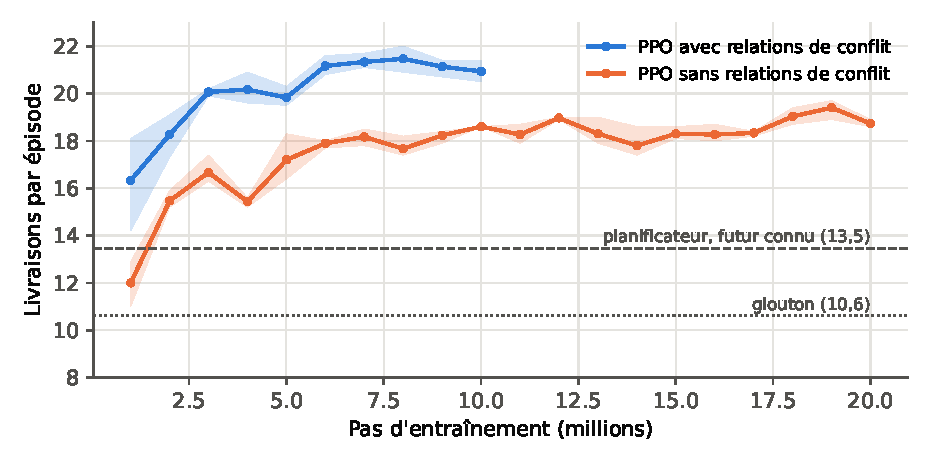
\includegraphics[width=0.75\linewidth]{figures/big.pdf}
\caption{Scénario big : livraisons par épisode pendant l'entraînement, avec et sans relations de conflit. Courbe : moyenne de trois graines. Bande : leur étendue. Chaque point est évalué sur 20 labyrinthes jamais vus. Lignes : glouton et planificateur, sur 100 labyrinthes.}
\label{fig:big}
\end{figure}

Avec les relations de conflit, PPO livre 21,30 caisses par épisode (21,0 à 21,7 selon la graine), deux fois plus que le glouton (10,61 ± 4,35). Sans elles, il plafonne entre 18,1 et 18,8, même après deux fois plus d'entraînement. Avec elles, il dépasse ce plafond dès 3 millions de pas. À budget presque égal (25 000 épisodes avec, 24 000 sans), l'écart est de 3,2 livraisons, alors que les trois graines ne s'écartent que d'une livraison au plus.

PPO dépasse aussi le planificateur, qui livre 13,12 caisses, et 13,47 s'il connaît l'avenir des humains. Celui-ci ne bloque jamais un autre robot, mais attend son tour sur les cases réservées par les autres. Ses trajets restent pourtant les plus directs. Son ratio de trajet, c'est-à-dire les actions par tâche divisées par le minimum nécessaire à un robot seul, vaut 1,20 à 1,27, contre 1,40 pour PPO et 2,12 pour le glouton. PPO ne fait donc pas des trajets plus courts : il en mène plus de front. Le glouton, lui, revient sur la case qu'il vient de quitter dans un tiers de ses déplacements, contre 5 \% pour PPO. Chaque pas change ce que voient ses rayons, et il hésite entre deux chemins.

\subsection{Approche décentralisée}

[À compléter par Juliette et Loïc.]

\section{Discussion et limites}

\subsection{Comparaison des deux approches}
[À compléter une fois les résultats de Juliette et Loïc disponibles : temps d'entraînement nécessaire, comportement face aux blocages, et ce que chaque approche gagne ou perd à mesure que la flotte grandit.]

\subsection{Approche centralisée}
Le contrôle centralisé tabulaire illustre concrètement la malédiction de la dimension~\cite{bellman1957} : l'espace d'états et d'actions est multiplié à chaque robot ajouté, et la table sature avant même d'avoir pu apprendre. PPO garde l'idée d'un contrôle commun à toute la flotte, mais remplace l'état joint par des caractéristiques propres à chaque robot et à ses relations avec les autres. C'est ce changement de représentation, plus que l'algorithme lui-même, qui permet de passer à l'échelle.

\subsection{Approche décentralisée}
[À compléter par Juliette et Loïc.]

\subsection{Limites}
Sur la carte 7x6, chaque configuration n'a été entraînée qu'avec une seule graine, faute de temps : les écarts entre PPO et le glouton (4 à 8 livraisons) dépassent largement le bruit d'évaluation (0,2 à 0,45 livraison), mais nous n'y avons pas mesuré la variance d'un entraînement à l'autre. Sur big, trois graines par configuration la bornent à une livraison. Les points intermédiaires de la figure~\ref{fig:big} ne portent que sur 20 labyrinthes, soit environ une livraison de bruit.

[Limites de l'approche décentralisée, à compléter par Juliette et Loïc.]

\subsection{Perspectives}
Une méthode comme QMIX~\cite{rashid2018}, qui combine des valeurs par robot en une valeur jointe, se situe entre la table centralisée et des apprenants indépendants, et permettrait de mesurer ce qu'apporte la coordination explicite. Ajouter une action « attendre » aiderait les robots à se céder le passage, à condition de casser la symétrie entre deux robots identiques qui choisiraient d'attendre en même temps.

\section{Conclusion}

Nous avons étudié la coordination d'une flotte de robots dans un entrepôt selon deux approches. Côté centralisé, la Q-table jointe sature dès 3 robots, tandis que PPO, en raisonnant robot par robot plutôt que sur l'état joint, dépasse une heuristique de plus court chemin à toutes les tailles de flotte, avec un écart qui croît avec la taille de la flotte, et généralise à des labyrinthes jamais vus : sur big, il livre 21,3 caisses contre 10,6 pour le glouton. Sans les relations de conflit entre robots, même deux fois plus d'entraînement ne comble pas l'écart. Ce résultat tient autant à des choix simples, mesurés un par un, qu'à l'algorithme : masquer les actions impossibles, donner au réseau la distance à sa cible plutôt que la carte entière, et lui signaler ses voisins immédiats.

[À compléter par Juliette et Loïc : conclusion sur l'approche décentralisée.]

[À compléter ensemble : laquelle des deux approches recommander, et dans quelles conditions.]

\begin{thebibliography}{9}

\bibitem{bellman1957}
R.~Bellman.
\newblock \emph{Dynamic Programming}.
\newblock Princeton University Press, 1957.

\bibitem{huang2022}
S.~Huang et S.~Ontañón.
\newblock A closer look at invalid action masking in policy gradient algorithms.
\newblock In \emph{Proceedings of the International FLAIRS Conference}, vol.~35, 2022.

\bibitem{rashid2018}
T.~Rashid, M.~Samvelyan, C.~Schroeder de Witt, G.~Farquhar, J.~Foerster et S.~Whiteson.
\newblock QMIX: Monotonic value function factorisation for deep multi-agent reinforcement learning.
\newblock In \emph{Proceedings of the 35th International Conference on Machine Learning (ICML)}, p.~4295--4304, 2018.

\bibitem{schulman2017}
J.~Schulman, F.~Wolski, P.~Dhariwal, A.~Radford et O.~Klimov.
\newblock Proximal policy optimization algorithms.
\newblock \emph{arXiv preprint arXiv:1707.06347}, 2017.

\bibitem{tan1993}
M.~Tan.
\newblock Multi-agent reinforcement learning: Independent vs.\ cooperative agents.
\newblock In \emph{Proceedings of the 10th International Conference on Machine Learning (ICML)}, p.~330--337, 1993.

\bibitem{watkins1992}
C.~J. C.~H. Watkins et P.~Dayan.
\newblock Q-learning.
\newblock \emph{Machine Learning}, 8(3--4):279--292, 1992.

\end{thebibliography}

\end{document}